\chapter{Conclusions}
% A plan of the work can be seen in \ref{fig:gantt}. The main bulk of the work after the literature review will be the creation of a quadruped robot, however, we have left a large amount of time into graph and data creation, and correct experiment development, as more work needs to go into developing a scientifically valid experiment for do gait generation. Although my plan does not currently contain a time allowance for getting a physical robot, we believe it would replace the time taken to implement other machine learning methods, as it is not an integral part of this dissertation.

% \begin{figure}[ht]
% 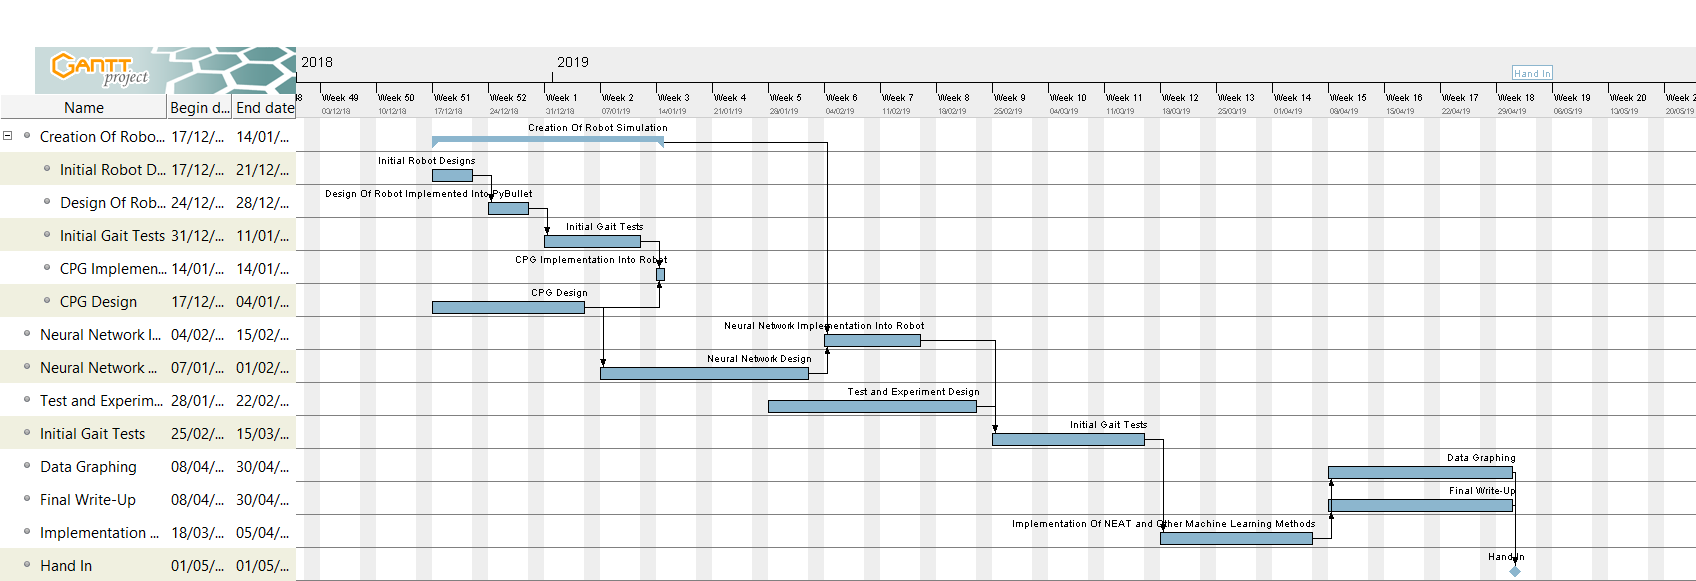
\includegraphics[width=15cm]{figures/gantt.png}
% \caption{A gantt chart showing the current project plan (www.ganttproject.biz)}
% \label{fig:gantt}
% \end{figure}

The work done in this paper provides a starting point for the creation of realistic animal gaits and additionally provides a platform through which other research may be done. As currently there does not exist an open source method of simulating and measuring animal gaits on quadrupeds, this research could provide a potential starting point for the development of realistic animal movements.

One of the main findings of this paper, was that irregardless of parameters tested, over 70\% of walking gaits performed tended within the amounts seen in the research of \cite{Alexander1983}. This shows that although it may be possible to 'cheat' evolutionary concepts and reach higher values than seen in evolutionary principles, to do so requires extremely fast repetition of gaits, which may be feasible in a step-simulation based environment, but might not apply to a real robot. 

This paper shows a valid initial breakdown of the effects of changing different parameter values on a simulated robot, with a valid comparison to Froude numbers found in mammals. This work additionally provides a basis for the measurement and creation of animal gaits, building a solid foundation from which other investigations can occur. 

Although this paper builds a foundation for the generation of simple gaits, only finds effective gait reproduction with walking gaits. This may be due to faster gaits requiring additional real-time feedback or methods of dynamic balancing. Similar issues have been found as in \cite{Rutishauser2008}, wherein a trotting gait does not produce gaits faster than walking. Although this research shows promising results for walking gaits, a more in depth study needs to be made for other gaits.